%% LyX 2.2.0alpha2 created this file.  For more info, see http://www.lyx.org/.
%% Do not edit unless you really know what you are doing.
\documentclass[english]{article}
\usepackage[T1]{fontenc}
\usepackage[latin9]{luainputenc}
\usepackage{geometry}
\geometry{verbose,tmargin=3cm,bmargin=3cm,lmargin=3cm,rmargin=3cm}
\usepackage{amsmath}
\usepackage{amssymb}
\usepackage{graphicx}

\makeatletter

%%%%%%%%%%%%%%%%%%%%%%%%%%%%%% LyX specific LaTeX commands.
%% Because html converters don't know tabularnewline
\providecommand{\tabularnewline}{\\}

%%%%%%%%%%%%%%%%%%%%%%%%%%%%%% User specified LaTeX commands.
\usepackage{fancyheadings}
\pagestyle{fancy}
\lhead{Kellen Betts}
\chead{videoMotionTrackingPCA}
\rhead{160731}

\makeatother

\usepackage{babel}
\begin{document}

\title{Motion Tracking in Video Data}

\author{Kellen Betts}

\date{Updated July 31, 2016}
\maketitle
\begin{abstract}
In this project, four experiments are used to develop an algorithm
for principal component analysis (PCA) with singular value decomposition
(SVD). We explore simple harmonic oscillations, pendulum motion, and
the effect of noise. The experimental apparatus is a paint can hanging
from a spring. The movement of the paint can is recorded by three
cameras. The video files from the cameras are processed to track the
location coordinates of the paint can over the course of the experiment.
PCA is used to extract the dynamical behavior from the data by reducing
redundancy and identifying the directions with maximal variance. In
the ideal case where the paint can oscillates in a single direction,
the PCA algorithm effectively isolates the behavior with a rank one
approximation. If noise is introduced by shaking the cameras, the
PCA algorithm is still able to isolate the oscillatory behavior but
with less accuracy. Finally, if the paint can oscillates in the vertical
direction and swings or rotates in the horizontal direction, the PCA
algorithm extracts the multidimensional behavior with expected rank
and reasonable accuracy.
\end{abstract}

\section{Introduction}

Four experiments are conducted using a paint can hanging from a spring.
The movement of the paint can is recorded by three independent cameras
(iPhones). The four experiments are:
\begin{enumerate}
\item \textbf{Test 1} (ideal case): A small displacement of the paint can
in the $z$ direction and the ensuing oscillations. In this case,
the entire motion is in the $z$ directions with simple harmonic motion
being observed.
\item \textbf{Test 2} (noisy case): Repeat the ideal case experiment, but
this time introduce camera shake into the video recording. This should
make it more difficult to extract the simple harmonic motion.
\item \textbf{Test 3} (horizontal displacement): In this case, the paint
can is released off-center so as to produce motion in the $x-y$ plane
as well as the $z$ direction. Thus, there is both a pendulum motion
and a simple harmonic oscillations.
\item \textbf{Test 4} (horizontal rotation): In this case, the mass is released
off-center and rotates so as to produce rotation in the $x-y$ plane
as well as oscillation in the $z$ direction. Thus, there is both
a pendulum motion and a simple harmonic oscillations.
\end{enumerate}
The primary objective in this project is to use principal component
analysis (PCA), where singular value decomposition (SVD) is a key
tool, to extract the dynamics of the paint can from the camera recordings
by reducing redundancy and identifying the directions of maximal variance.
The location of the paint can is tracked in each video by isolating
a target color on the can and logging its coordinates in each frame.
The coordinates from each video in a particular experiment are then
compiled into a matrix that comprises the data used in the PCA algorithm.

\section{Theoretical Background}

The governing equation for this system is known,
\begin{equation}
\frac{d^{2}f}{dt^{2}}=-\omega^{2}f
\end{equation}
where $f\left(t\right)$ measures the displacement of the mass in
the vertical direction. Equation 1 has the analytical solution,
\begin{equation}
f\left(t\right)=A\,\cos\left(\omega t+\omega_{0}\right)
\end{equation}
The primary objective is to identify the motion of the paint can using
PCA by removing redundancy and identifying the maximal variance in
the data. In the first experiment there is one degree of freedom with
the paint can oscillating in the vertical direction. However, the
experimental setup includes three streams of data collecting locations
of the paint can in two directions. This means there is a lot of redundancy
in the incoming data. 

Variance for a dataset $\vec{a}=\left(a_{1},\,a_{2},\,\ldots,\,a_{n}\right)$
is calculated by,
\begin{equation}
\sigma_{a}^{2}=\frac{1}{n-1}\vec{a}\vec{a}^{T}
\end{equation}
and correlation between two datasets $\vec{a}$ and $\vec{b}$ is
calculated by the covariance,
\begin{equation}
\sigma_{ab}^{2}=\frac{1}{n-1}\vec{a}\vec{b}^{T}
\end{equation}
If two vectors are orthogonal then their dot product is zero, and
so their covariance is zero. Conversely, if the dot product is large
and thus the covariance is large then the two vectors are related.
Therefore, covariance provides a measure of statistical dependency
between two datasets. 

For a matrix,
\begin{equation}
X\;\epsilon\;\mathbb{R}^{m\times n}
\end{equation}
the covariance matrix is calculated,
\begin{equation}
C_{x}=\frac{1}{n-1}XX^{T}
\end{equation}
which can be written,
\begin{equation}
C_{x}=\begin{bmatrix}\sigma_{x,a}^{2} & \sigma_{x,y,a}^{2} & \sigma_{x,x,a,b}^{2} & \cdots\\
\vdots & \sigma_{y,a}^{2}\\
 &  & \sigma_{x,b}^{2}\\
 &  &  & \ddots\\
 &  &  &  & \sigma_{y,c}^{2}
\end{bmatrix}\;\epsilon\;\mathbb{R}^{m\times m}
\end{equation}
The diagonal of the covariance matrix contains the variance of each
data stream and the off-diagonals contain the covariance between pairs
of the streams. This means the off-diagonals contain information about
redundancy in the data. Moreover, since dynamical behavior is characterized
by change and covariance is a measure of change between two data streams,
then covariance(s) provides a measure of dynamical behavior in a given
dataset. In this project, three cameras are capturing data of the
same apparatus and so covariance provides a way to identify the dynamics
of the paint can from the video data.

For the matrix $X$ (equation 5), the singular value decomposition
(SVD) is defined,
\begin{equation}
X=U\Sigma V^{*}
\end{equation}
where $\Sigma$ is a diagonal matrix of singular values $\sigma$
that correspond to the square root of the eigenvalues $\left(\sigma_{i}=\sqrt{\lambda_{i}}\right)$
and are ordered based on size. $U$ and $V^{*}$ are orthonormal unitary
transformations corresponding to the orientation of the incoming data.
Using the proper orthogonal modes from the SVD, a low rank approximation
can be calculated by the sum,
\begin{equation}
X_{N}\approx\sum_{j=1}^{N}\sigma_{j}\vec{u}_{j}\vec{v^{*}}_{j}
\end{equation}
where $N$ is a given rank. The 2-norm error for the approximation
is given by,
\begin{equation}
\left\Vert X-X_{N}\right\Vert _{2}=\sigma_{n+1}\,.
\end{equation}
One way to think about SVD is as a least squares fit in higher dimensional
space where the elements of $\Sigma$ are ordered by their $L^{2}$
energy. The energy for a given mode can be calculated,
\begin{equation}
\mathrm{energy}_{i}=\frac{\sum_{i=1}^{N}\sigma_{i}}{\sum_{i=1}^{n}\sigma_{i}}\,.
\end{equation}
Therefore, diagonalization with SVD is a transformation to a new orthonormal
basis and provides low rank approximation for a given dataset. To
diagonalize the covariance matrix the transformation variable $Y$
is defined,
\begin{equation}
Y=U^{*}X
\end{equation}
and the variance in $Y$ (see Appendix C for derivation) is calculated,
\begin{equation}
C_{Y}=\frac{1}{n-1}\Sigma^{2}\,.
\end{equation}
In this form the system is said to be written in terms of its principal
components with the diagonal matrix $\Sigma^{2}$ containing variance
measures in $Y$ ordered based by size. This means that the dominant
$\sigma_{i}^{2}$ values reflect directions of maximal variance and
allow a low rank approximation of the spatiotemporal dynamics in the
data.

\section{Algorithm Implementation and Development}

\subsection{Position Measurements:}

After importing the video data and extracting the data for a given
frame, the first task is to identify the $x,y$ coordinates of the
paint can in the frame. Initially, I attempted to implement a tracking
algorithm that got coordinates for the light on the top of the can
by brightness. Based on the suggestion from the Catalyst discussion
board (megan970), I modified the algorithm to track the yellow color
on the paint can. There are five steps in the tracking algorithm that
are repeated for each frame in a video:
\begin{enumerate}
\item Choosing target color
\item Getting individual frame
\item Building difference image
\item Identifying location of target color
\end{enumerate}
The RGB values for the yellow color on the paint can are manually
identified using a separate image editing application similar to Photoshop.
Since the color spectrum is different for each of the videos, a subroutine
$\mathtt{targetColor.m}$ is used to match RGB values to video. A
given video is then passed into a loop that will process each frame.
Inside the loop, the frame is converted to an image and double precision
format. Each color channel is then isolated and the target color value
for the channel is subtracted off. The color channels are then combined
into a 2-norm difference image where brightness reflects the distance
from the target color. As seen in Figure 1, the target color takes
a zero intensity value (black) and the rest of the image scales to
reflect the difference from the target color. Using this difference
image, the paint can location is identified (Figure 2) by finding
the coordinates of the minimum value (i.e. the location of the pixel
that is closest to the target color). For each camera, the location
of the paint can is collected in vectors $\left(\vec{x}_{i}\,,\,\vec{y}_{i}\right)$.
The data is then arranged into the matrix,
\begin{equation}
X=\begin{bmatrix}\vec{x}_{a}\\
\vec{y}_{a}\\
\vec{x}_{b}\\
\vec{y}_{b}\\
\vec{x}_{c}\\
\vec{y}_{c}
\end{bmatrix}\;\epsilon\;\mathbb{R}^{m\times n}
\end{equation}
where $\,i=a,\,b,\,c$ are the three cameras, $m$ is the number of
``sensors'' tracking the paint can location, and $n$ corresponds
to the number of measurements in time (meaning the length of the video).
In these experiments, the location is tracked in $\left(x,y\right)$
for three camera and so the $m=6$. Once data for the paint can location
is obtained for each of the cameras in a given test scenario, the
final task is to synchronize the first frames and trim the data to
the length of the shortest video so that covariances between the videos
can be calculated.

To speed processing, the use of cropping to the region containing
the motion of the paint can is explored (Figure 2). The challenge
with using cropping is the effort to manually identifying the region
in each video that contains the entire range of motion of the paint
can. The observed run time using cropped images is approximately twice
as fast due to the data reduction, however, nearly identical results
are obtained for the paint can location from both cropped and uncropped
videos. Therefore, to reduce the upfront manual workload and prevent
potential error from cropping out necessary information, all further
analyses use uncropped videos. 

\noindent \vspace{0.07\paperheight}

\begin{center}
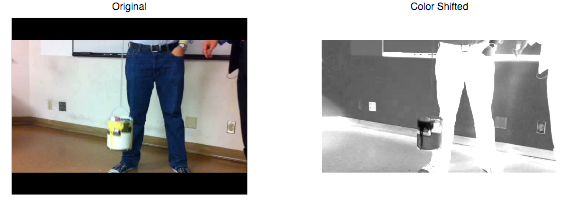
\includegraphics[width=1\columnwidth]{plots/test2_colorShift_noCrop}\textbf{}\\
\textbf{}%
\begin{minipage}[t]{0.75\columnwidth}%
\textbf{Figure 1.} For a specified target color (in this case the
yellow on the paint can), a difference image is constructed using
the 2-norm of the difference from the target color. This creates an
image (right) where the target color takes the minimum value and the
rests of the image is scaled by difference from the target color.%
\end{minipage}
\par\end{center}

\noindent \begin{center}
\pagebreak{}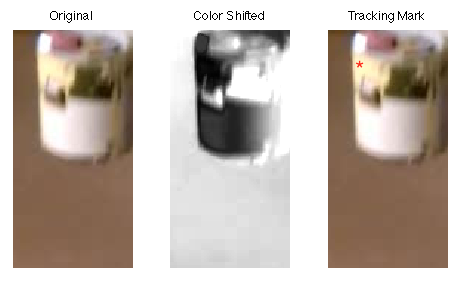
\includegraphics[width=0.65\columnwidth]{plots/test1_colorShift_crop}\textbf{}\\
\textbf{}%
\begin{minipage}[t]{0.75\columnwidth}%
\textbf{Figure 2.} The paint can location (right) is identified by
finding the minimum value in the difference image (center) where the
scale is based on the difference from the target color (yellow on
the can).%
\end{minipage}
\par\end{center}

\noindent \vspace{0.02\paperheight}


\subsection{Principal Component Analysis:}

There are three steps in the PCA algorithm:
\begin{enumerate}
\item Subtracting the mean from the data
\item SVD of the data
\item Output/visualization of results
\end{enumerate}
Implementation is greatly simplified because calculation of the mean
and the SVD operation are performed using built in MATLAB functions
(see Appendix A). The outputs from the $\mathtt{svd()}$ function
are the $U,\,\Sigma,\,V^{*}$ matrices. The principal component projections
$\left(Y=U^{*}X\right)$, diagonal variances $\left(\sigma_{i}^{2}=\lambda_{i}\right)$,
and proper orthogonal modes (equation 9) are plotted in the subroutine
$\mathtt{plotProjections.m}$. The energy contained at a given mode
is calculated using equation 11.

\section{Computational Results}

\subsection{Test 1}

In Test 1, the paint can is set to oscillate in a purely vertical
direction and so we should expect maximal variance in one component.
Plotting the raw location tracking data (Figure 3) clearly shows consistent
oscillation in the vertical direction and minimal movement in the
horizontal for all three cameras. Energies of the diagonal variances
from the PCA were,

\noindent \begin{center}
\begin{tabular}{|c|c|c|c|c|c|c|}
\hline 
$\sigma_{i}^{2}$ & 1 & 2 & 3 & 4 & 5 & 6\tabularnewline
\hline 
\hline 
energy & 0.9499 & 0.9744 & 0.9874 & 0.9959 & 0.9986 & 1.0000\tabularnewline
\hline 
\end{tabular}
\par\end{center}

\noindent indicating that \textasciitilde{}95\% of the variance are
captured in the first principal component. Figure 4 shows that the
variance in the first component is almost $10^{2}$ greater than the
others. Plotting of the principal component projections (Figure 5)
and the proper orthogonal modes (Figure 6) confirm that the first
component or the rank one approximation captures the one dimensional
oscillation in this test case.

\noindent \begin{center}
\pagebreak{}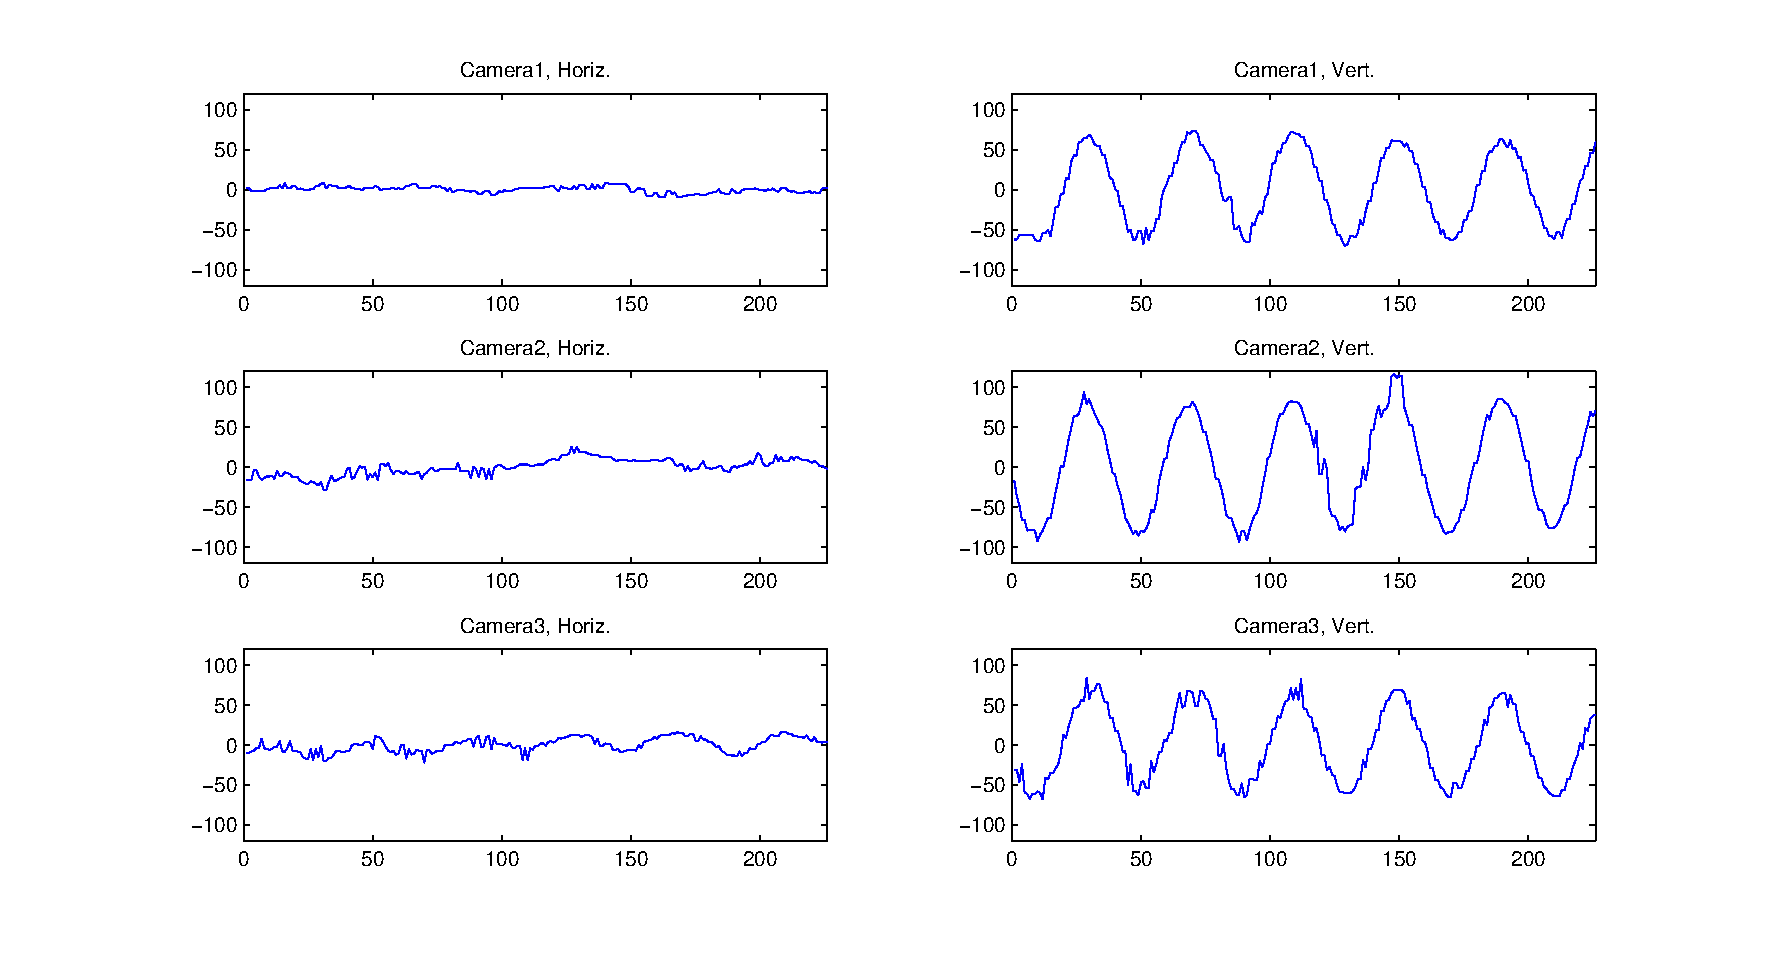
\includegraphics[width=1\columnwidth]{plots/test1_tracking}\textbf{}\\
\textbf{}%
\begin{minipage}[t]{0.75\columnwidth}%
\textbf{Figure 3.} For Test 1, the raw location tracking data for
each camera clearly shows oscillation in the vertical (right) direction
and minimal movement in the horizontal (left).%
\end{minipage}
\par\end{center}

\noindent \begin{center}
\vspace{0.08\paperheight}
\par\end{center}

\noindent \begin{center}
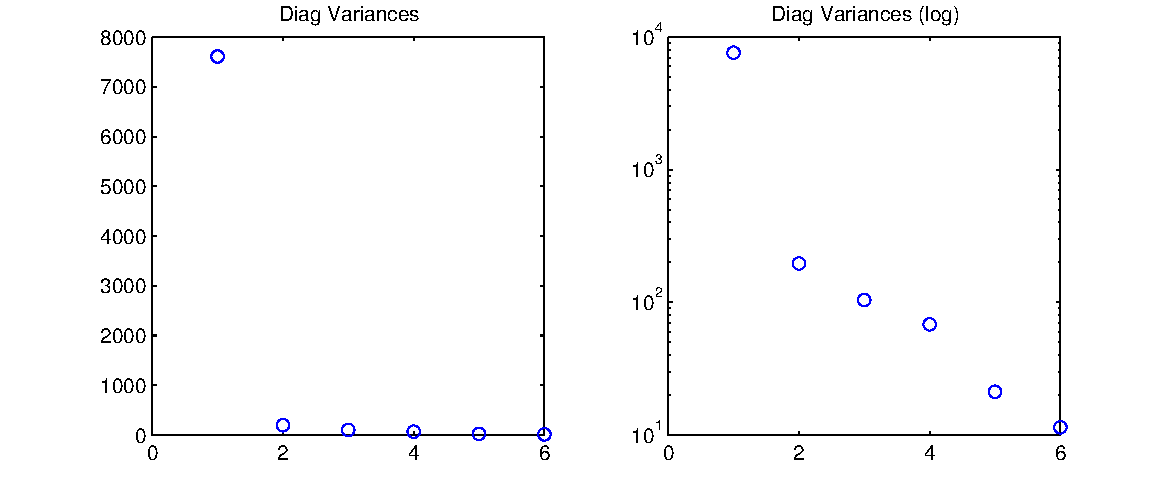
\includegraphics[width=1\columnwidth]{plots/test1_variance_before}\textbf{}\\
\textbf{}%
\begin{minipage}[t]{0.75\columnwidth}%
\textbf{Figure 4.} For Test 1, the diagonal variances $\left(\sigma_{i}^{2}=\lambda_{i}\right)$
show that the first component captures most of the variance with almost
$10^{2}$ more variance than the others. %
\end{minipage}
\par\end{center}

\noindent \begin{center}
\pagebreak{}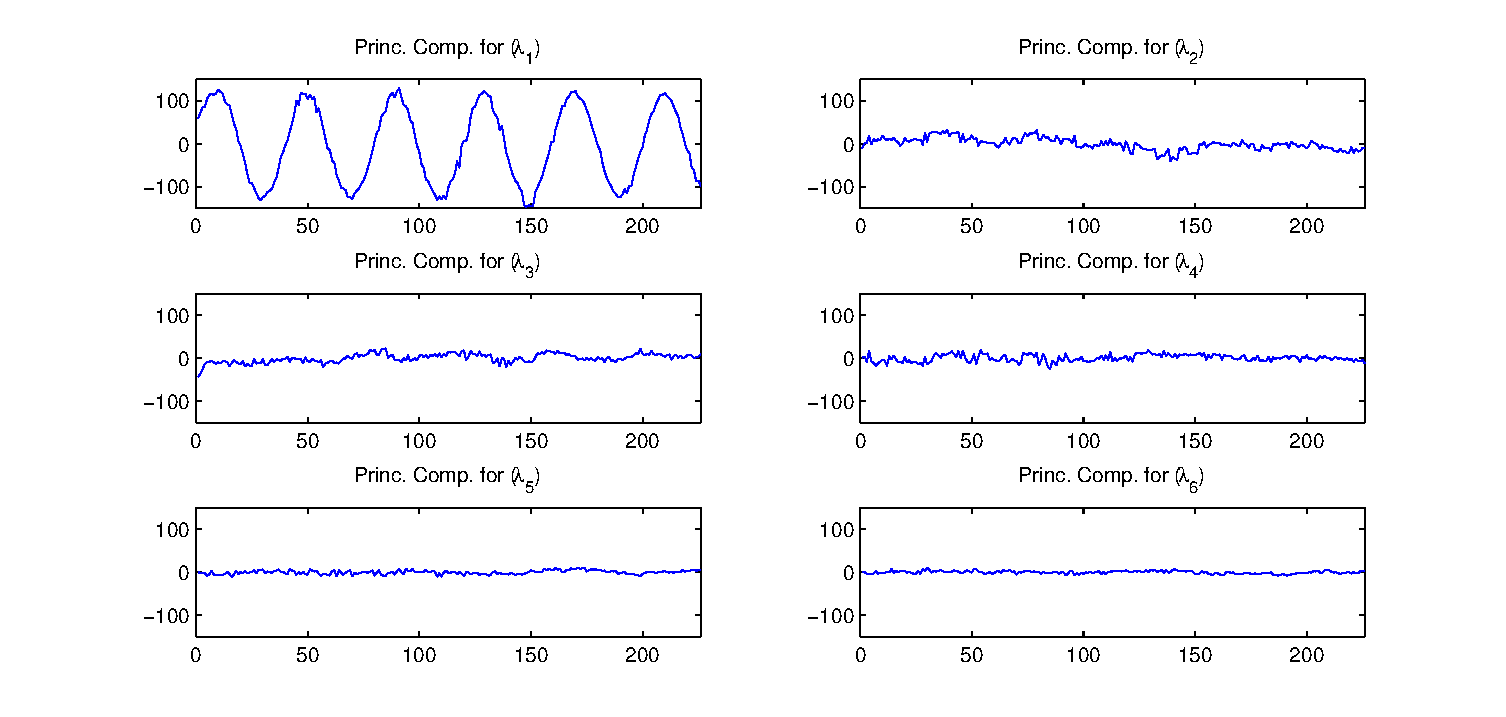
\includegraphics[width=0.95\columnwidth]{plots/test1_princComp}\textbf{}\\
\textbf{}%
\begin{minipage}[t]{0.75\columnwidth}%
\textbf{Figure 5.} For Test 1, the principal components $\left(Y\right)$
shows that the first component (top left) clearly captures the oscillatory
behavior of the can.%
\end{minipage}\vspace{0.005\paperheight}
\par\end{center}

\noindent \begin{center}
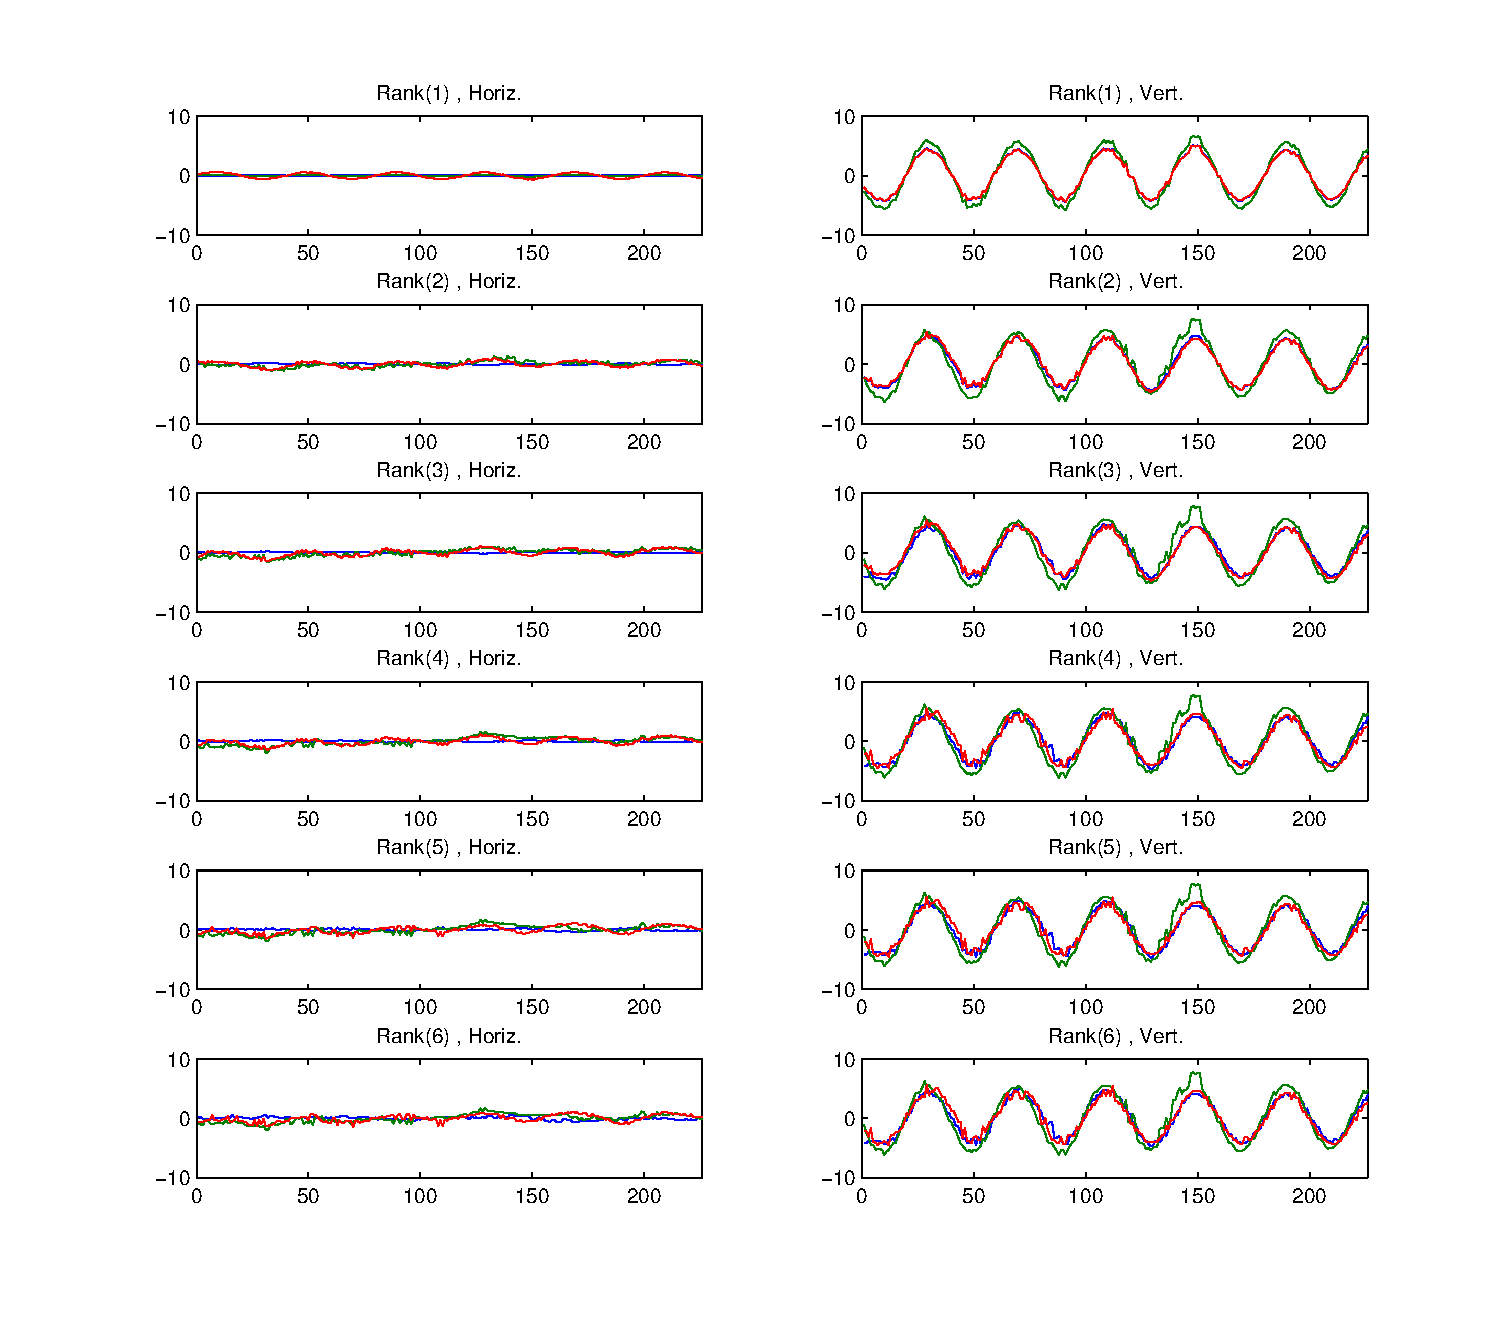
\includegraphics[width=0.85\columnwidth]{plots/test1_modes_before}\textbf{}\\
\textbf{}%
\begin{minipage}[t]{0.75\columnwidth}%
\textbf{Figure 6.} For Test 1, the proper orthogonal modes shows that
a rank one approximation (first row) captures that vertical (right)
oscillatory behavior and is a close match to the full rank (bottom
row) data.%
\end{minipage}
\par\end{center}

\noindent \begin{center}
\pagebreak{}
\par\end{center}

\subsection{Test 2}

In Test 2, the paint can is set to oscillate in a purely vertical
direction just as in Test 1 and so we should expect maximal variance
in one component. However, the camera operators intentionally shook
the camera while recording introducing noise in the data. The intention
of this scenario is to explore how noise affects the PCA algorithm.
Plotting the raw location tracking data (Figure 7) shows oscillation
in the vertical direction that is consistent but much more erratic
than Test 1. The horizontal direction shows some movement but no consistent
oscillatory behavior. Therefore, the noise from the camera shake diminishes
the quality of the data in both the horizontal and vertical directions.
Energies of the diagonal variances from the PCA were,

\noindent \begin{center}
\begin{tabular}{|c|c|c|c|c|c|c|}
\hline 
$\sigma_{i}^{2}$ & 1 & 2 & 3 & 4 & 5 & 6\tabularnewline
\hline 
\hline 
energy & 0.6527 & 0.8079 & 0.8985 & 0.9468 & 0.9796 & 1.0000\tabularnewline
\hline 
\end{tabular}
\par\end{center}

\noindent indicating that only \textasciitilde{}65\% of the variance
is captured in the first principal component compared to \textasciitilde{}95\%
for Test 1. Figure 8 shows that the variance in the first component
is dominant but has less than $10^{1}$ more variance than the others.
Plotting the principal component projections (Figure 9) shows that
both the first and second components show oscillatory behavior. The
proper orthogonal modes (Figure 10) confirm that a rank one approximation
does capture the vertical oscillation, but the rank four approximation
(corresponding to \textasciitilde{}95\% energy) is a better match
to the full rank (six) data. These results indicate that the noise
from the camera shake diminishes performance.

\noindent \begin{center}
\vspace{0.05\paperheight}
\par\end{center}

\noindent \begin{center}
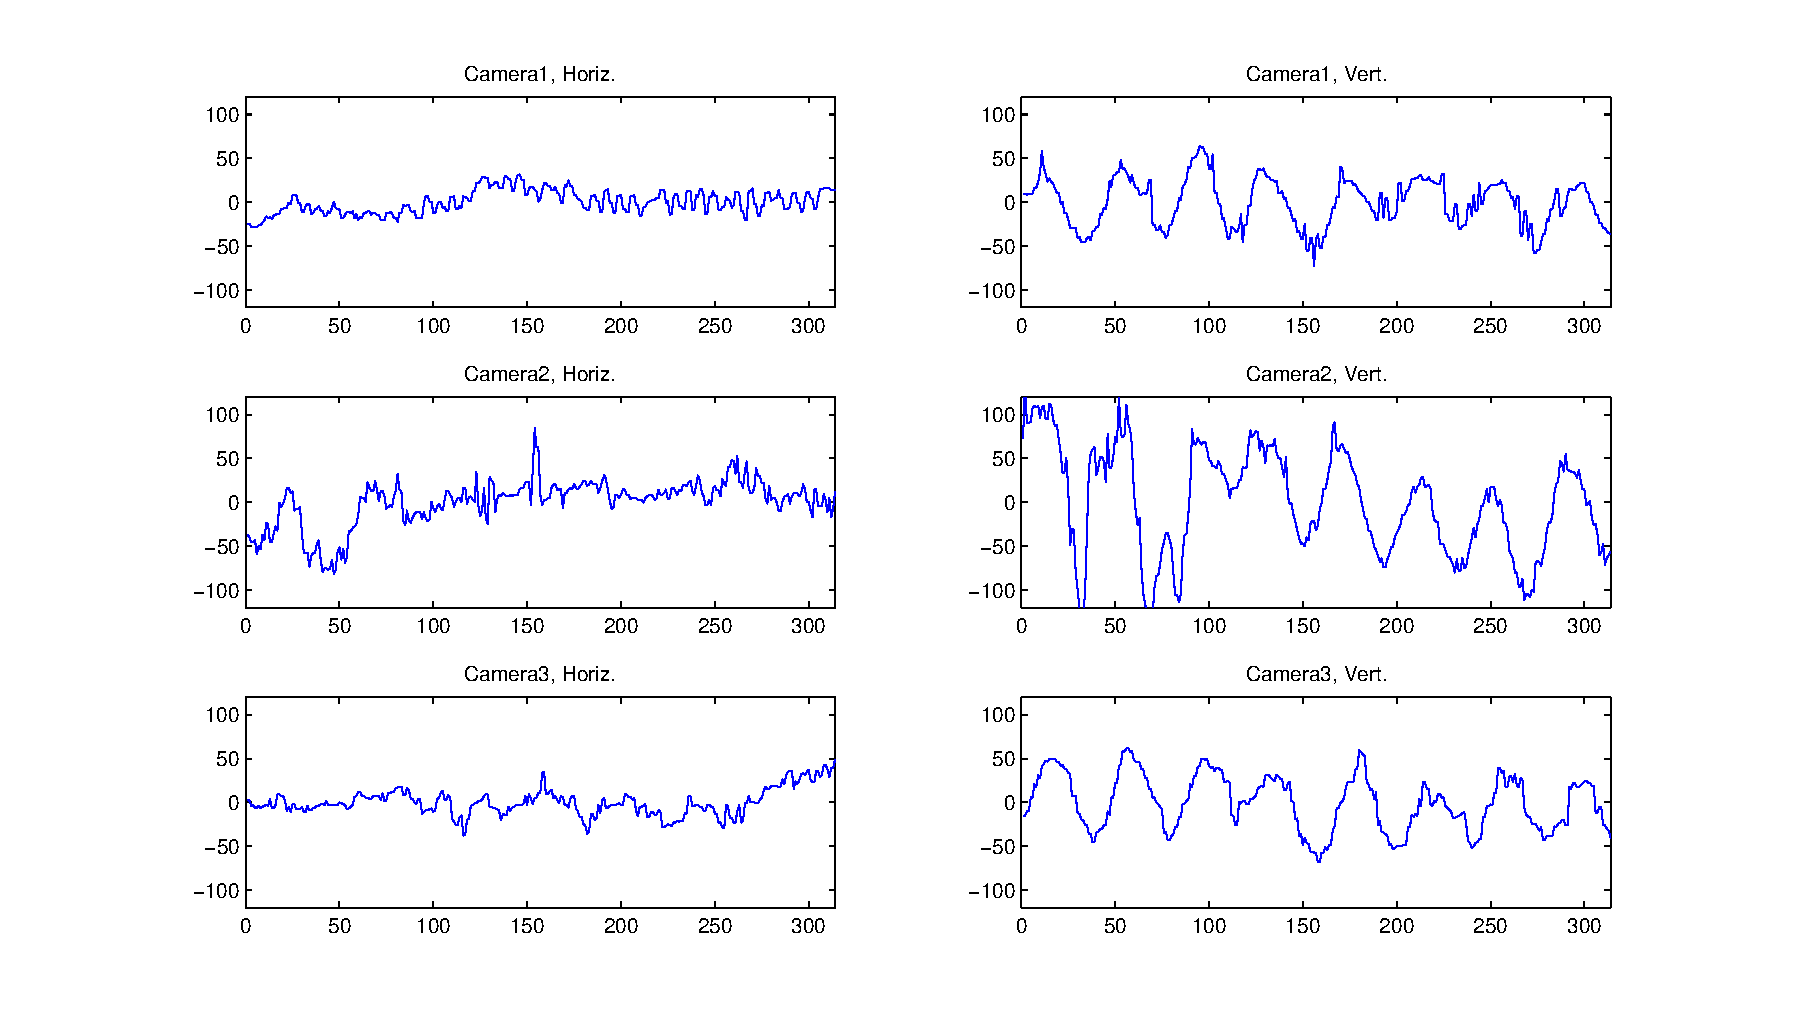
\includegraphics[width=1\columnwidth]{plots/test2_tracking}\textbf{}\\
\textbf{}%
\begin{minipage}[t]{0.75\columnwidth}%
\textbf{Figure 7.} For Test 2, the raw location tracking data for
each camera clearly shows oscillation in the vertical (right) direction
but the noise-inducing camera shake diminishes its consistency and
introduces movement in the horizontal direction (left).%
\end{minipage}
\par\end{center}

\noindent \begin{center}
\pagebreak{}
\par\end{center}

\noindent \begin{center}
\vspace{0.03\paperheight}
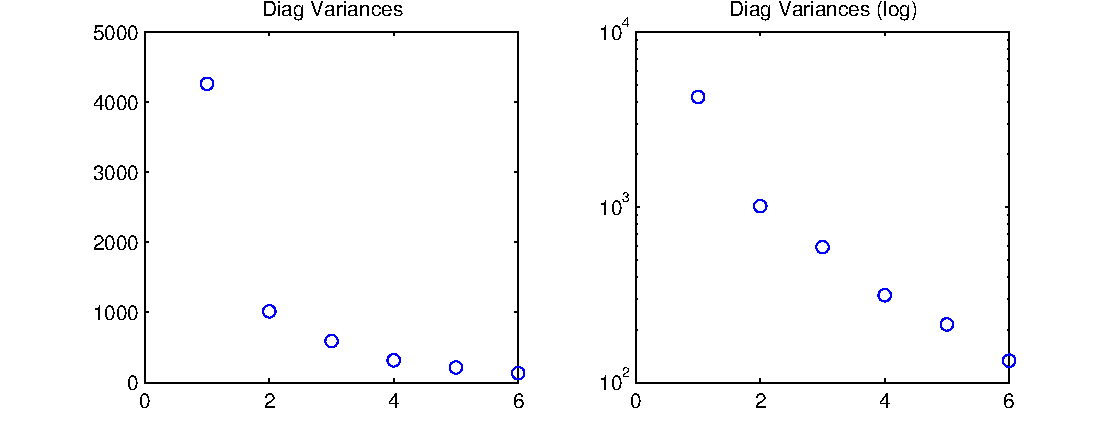
\includegraphics[width=1\columnwidth]{plots/test2_variance}\textbf{}\\
\textbf{}%
\begin{minipage}[t]{0.75\columnwidth}%
\textbf{Figure 8.} For Test 2, the diagonal variances $\left(\sigma_{i}^{2}=\lambda_{i}\right)$
show that the first component is dominant but less than $10^{1}$
more than the others. %
\end{minipage}\vspace{0.1\paperheight}
\par\end{center}

\noindent \begin{center}
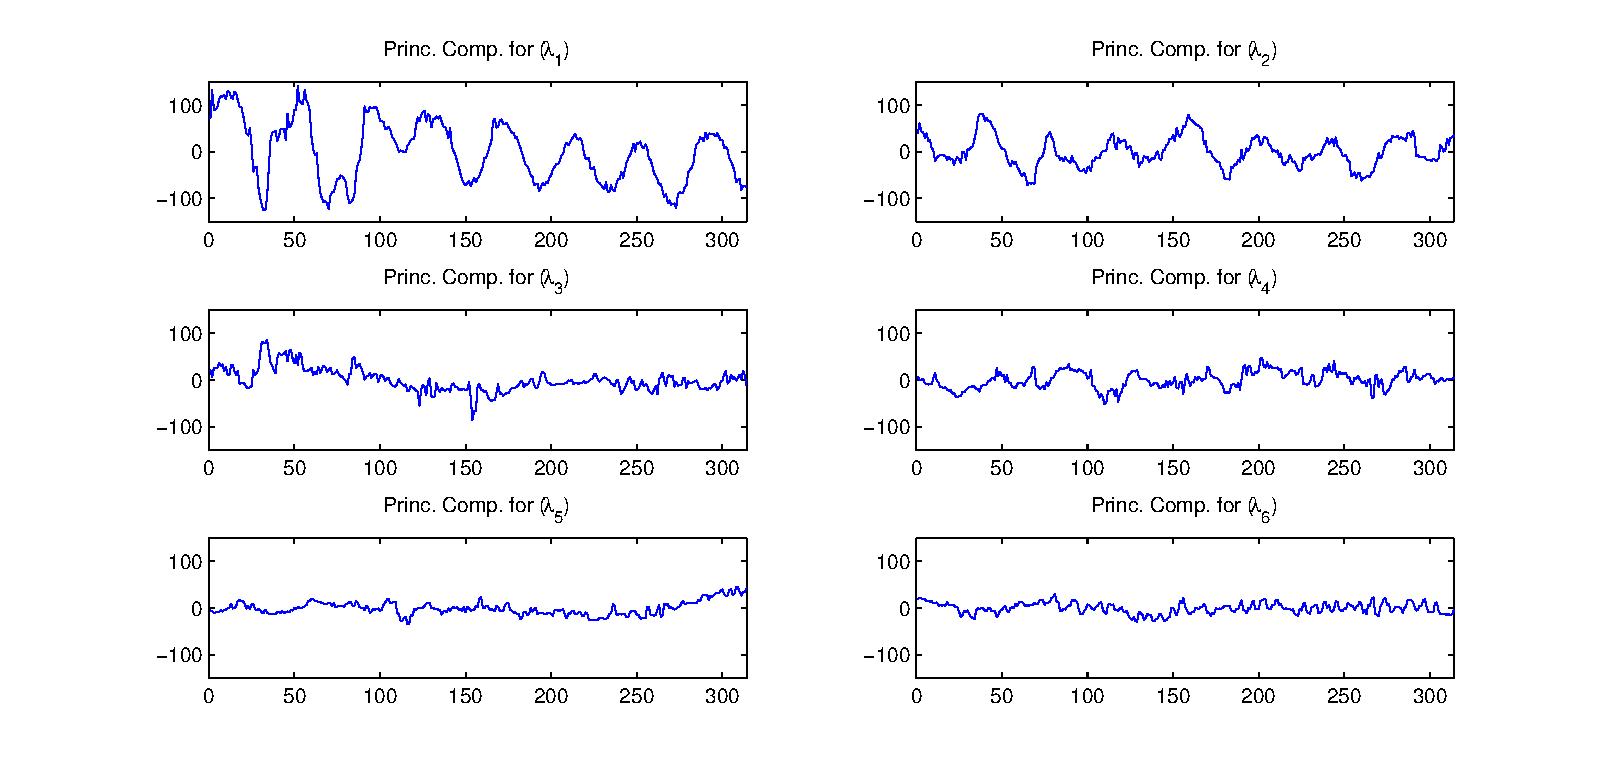
\includegraphics[width=1\columnwidth]{plots/test2_princComp}\textbf{}\\
\textbf{}%
\begin{minipage}[t]{0.75\columnwidth}%
\textbf{Figure 9.} For Test 2, the principal component projections
$\left(Y\right)$ shows that both the first and second components
show oscillatory behavior.%
\end{minipage}\pagebreak{}
\par\end{center}

\noindent \begin{center}
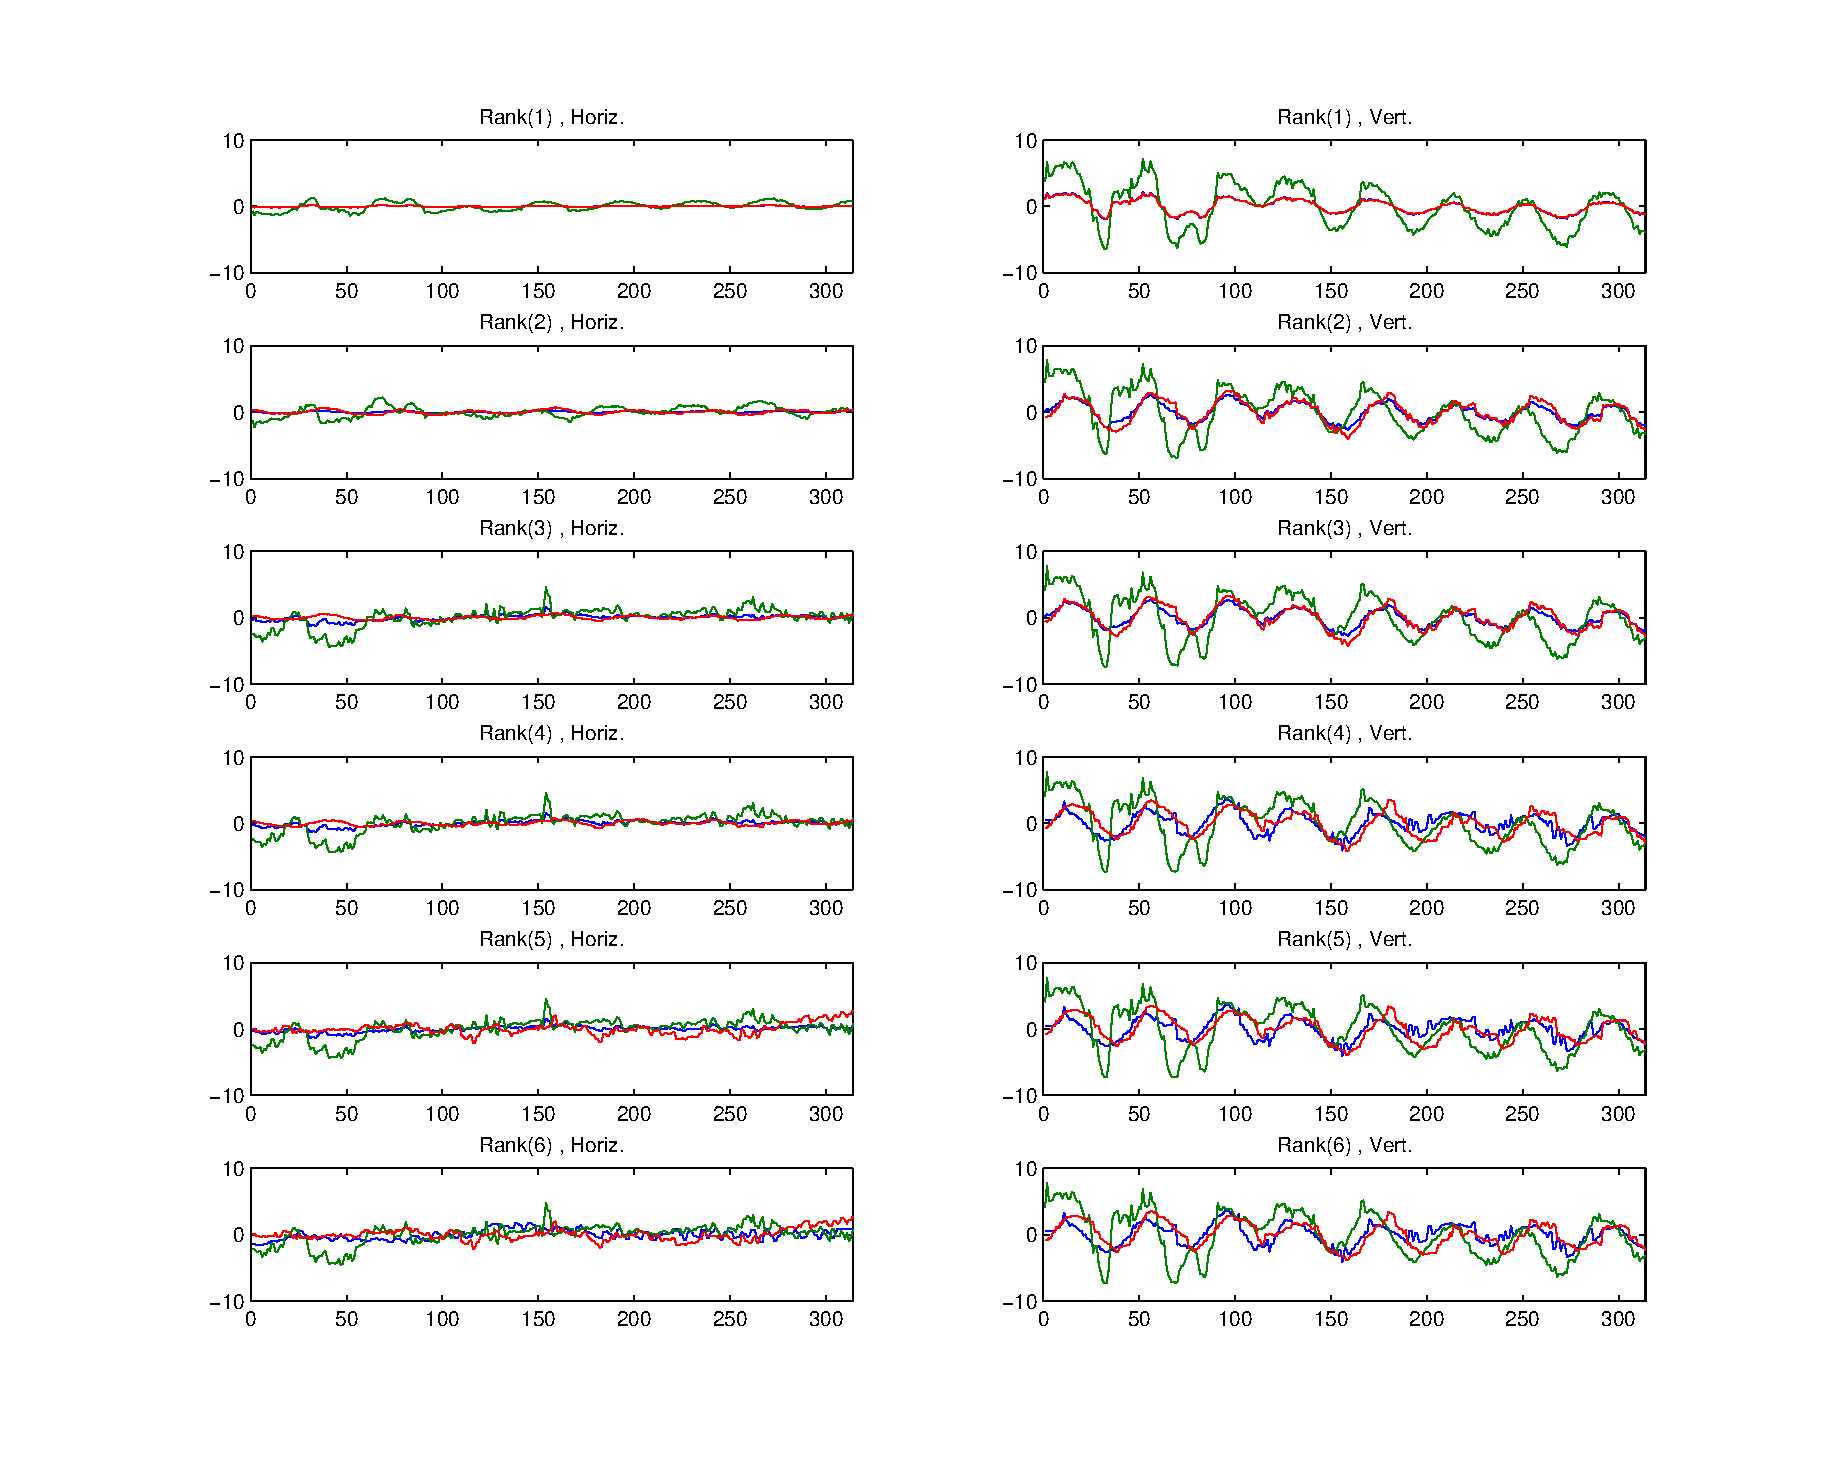
\includegraphics[width=0.85\columnwidth]{plots/test2_modes}\textbf{}\\
\textbf{}%
\begin{minipage}[t]{0.75\columnwidth}%
\textbf{Figure 10.} For Test 2, the proper orthogonal modes show that
a rank one approximation does capture vertical oscillation, but the
rank four approximation (forth from top) is a better match to the
full rank (bottom row).%
\end{minipage}
\par\end{center}

\noindent \begin{center}
\vspace{0.02\paperheight}
\par\end{center}

\subsection{Test 3}

In Test 3, the paint can is set to oscillate in the vertical direction
just as in Test 1-2 but is also set to oscillate in the horizontal
direction and so we should expect maximal variance for two components.
Plotting the raw location tracking data (Figure 11) shows oscillation
in both the vertical and horizontal directions for all three cameras. 

Energies of the diagonal variances from the PCA were,

\noindent \begin{center}
\begin{tabular}{|c|c|c|c|c|c|c|}
\hline 
$\sigma_{i}^{2}$ & 1 & 2 & 3 & 4 & 5 & 6\tabularnewline
\hline 
\hline 
energy & 0.4756 & 0.7226 & 0.9009 & 0.9580 & 0.9957 & 1.0000\tabularnewline
\hline 
\end{tabular}
\par\end{center}

\noindent indicating that \textasciitilde{}48\% of the variance is
captured in the first principal component, \textasciitilde{}72\% in
the second, and that it takes four modes to reach 95\%. Figure 12
shows that the variance in the first component is dominant but that
the trend is approximately linear for the first five modes. Plotting
the principal component projections (Figure 13) shows that the first
three components contain oscillatory behavior. The proper orthogonal
modes (Figure 14) show that a rank two approximation captures the
vertical and horizontal oscillation, but the rank four approximation
(corresponding to \textasciitilde{}95\% energy) is a better match
to the full rank (six) data. These results indicate that the the PCA
algorithm effectively captures the horizontal and vertical oscillation
with two components, but better accuracy is achieved with higher rank
data.\pagebreak{}

\noindent \begin{center}
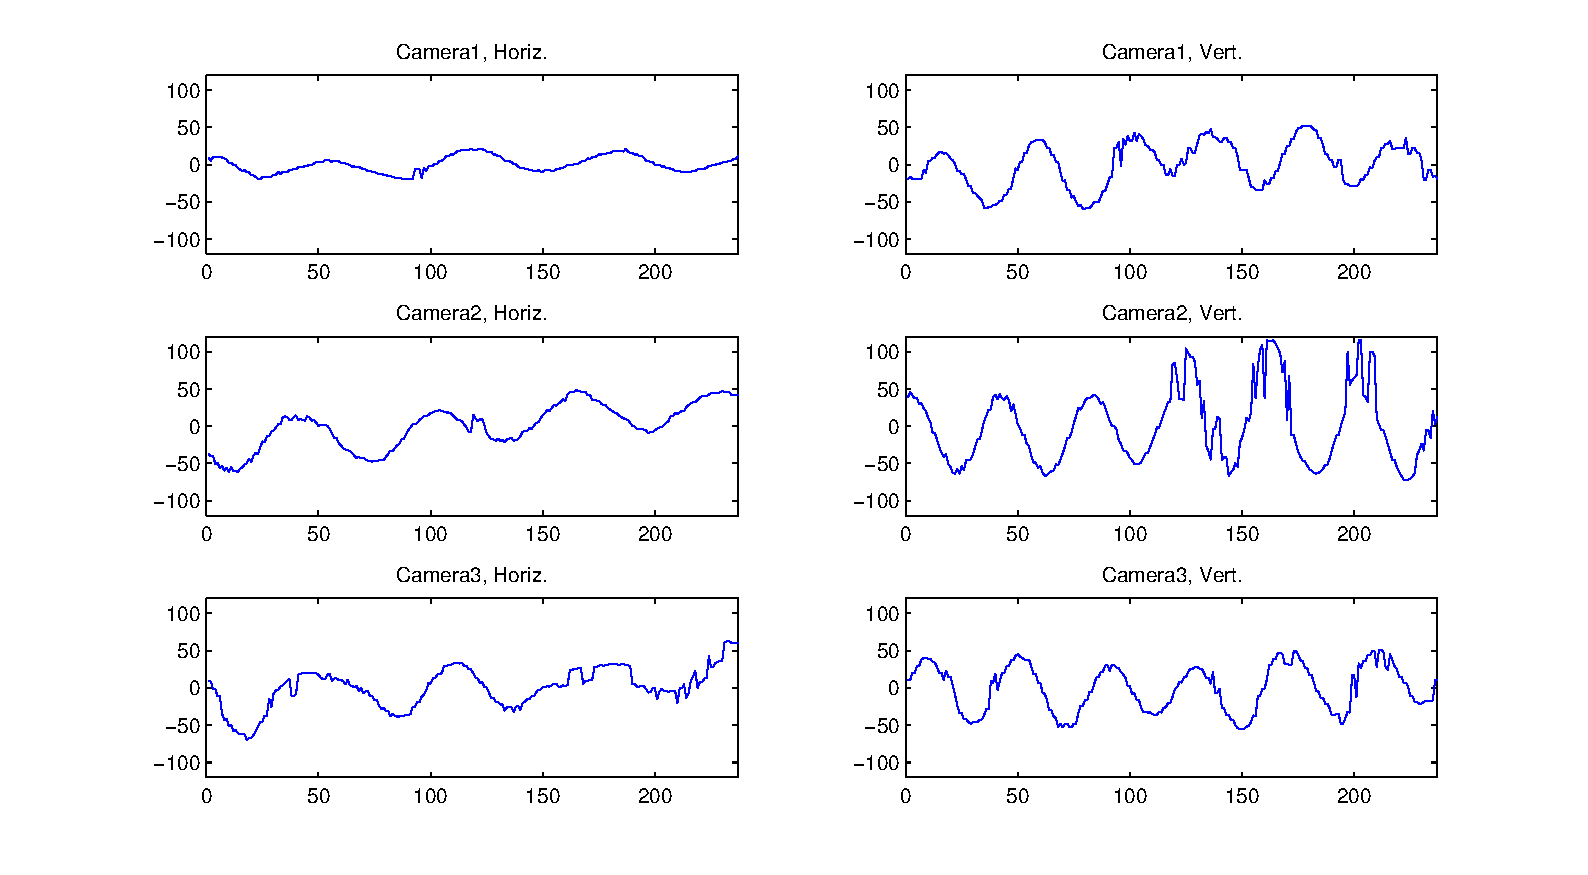
\includegraphics[width=1\columnwidth]{plots/test3_tracking}\textbf{}\\
\textbf{}%
\begin{minipage}[t]{0.75\columnwidth}%
\textbf{Figure 11.} For Test 3, the raw location tracking data clearly
shows oscillation in both the vertical (right) and horizontal (left)
directions for all three cameras.%
\end{minipage}
\par\end{center}

\noindent \begin{center}
\vspace{0.06\paperheight}
\par\end{center}

\noindent \begin{center}
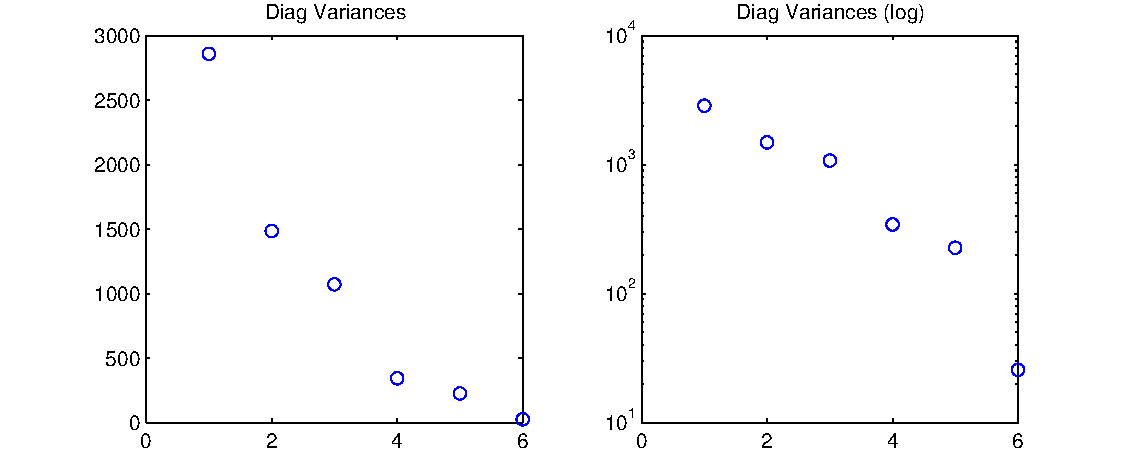
\includegraphics[width=1\columnwidth]{plots/test3_variance}\textbf{}\\
\textbf{}%
\begin{minipage}[t]{0.75\columnwidth}%
\textbf{Figure 12.} For Test 3, the diagonal variances $\left(\sigma_{i}^{2}=\lambda_{i}\right)$
show that the variance in the first component is dominant but that
the trend is approximately linear for the first five modes. %
\end{minipage}
\par\end{center}

\noindent \begin{center}
\pagebreak{}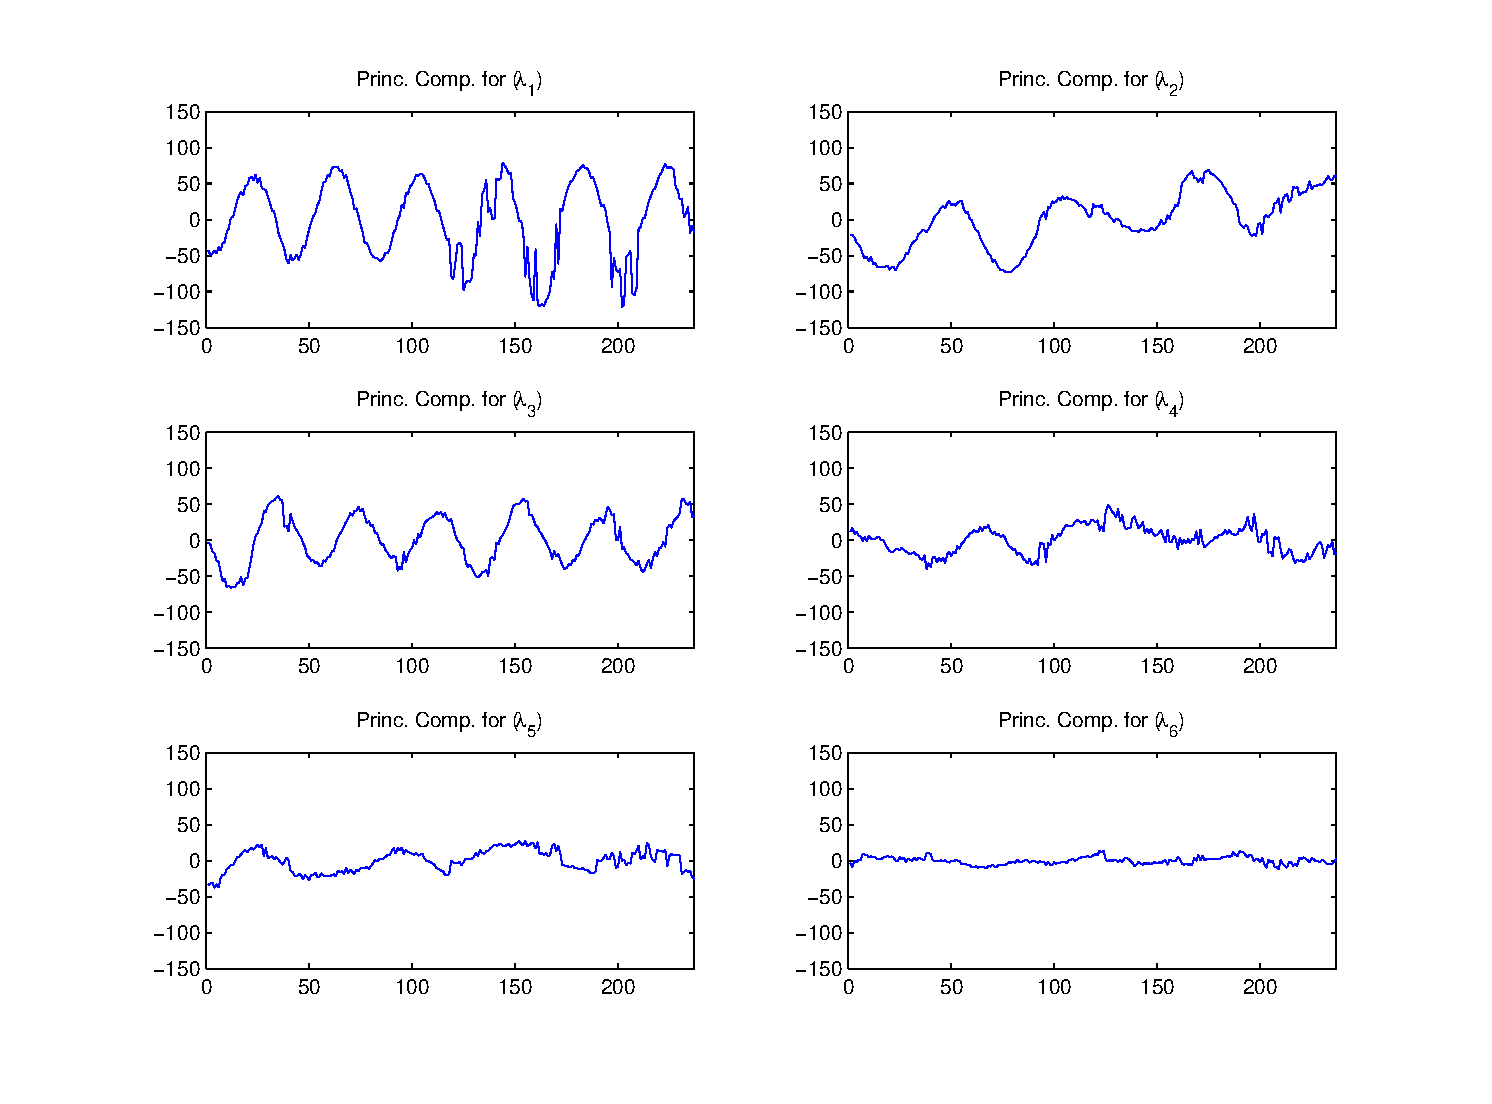
\includegraphics[width=0.78\columnwidth]{plots/test3_princComp}\textbf{}\\
\textbf{}%
\begin{minipage}[t]{0.75\columnwidth}%
\textbf{Figure 13.} For Test 3, the principal component projections
$\left(Y\right)$ shows that the first three components contain oscillatory
behavior.%
\end{minipage}
\par\end{center}

\noindent \begin{center}
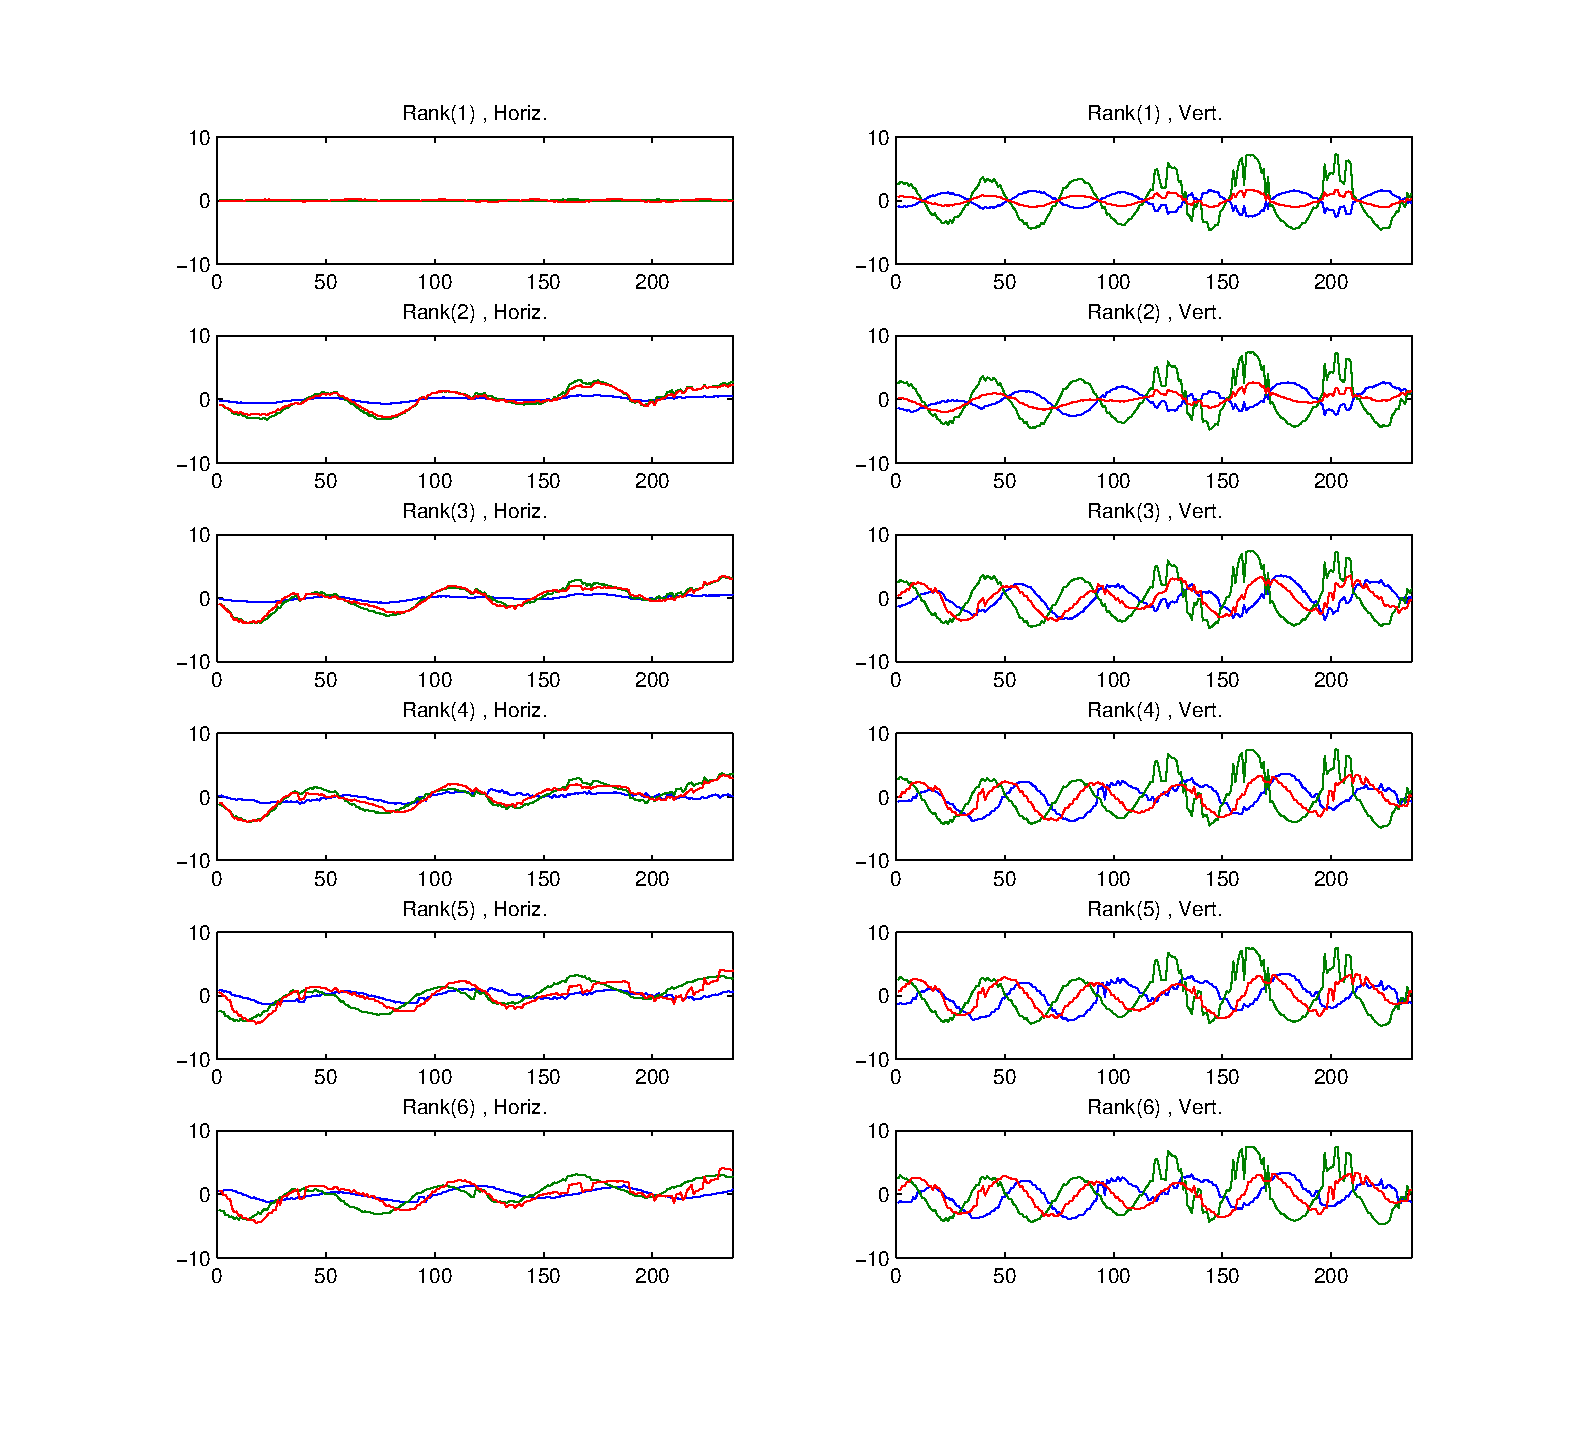
\includegraphics[width=0.75\columnwidth]{plots/test3_modes}\\
\textbf{}%
\begin{minipage}[t]{0.75\columnwidth}%
\textbf{Figure 14.} For Test 3, the proper orthogonal modes show that
rank two (second from top) captures the vertical and horizontal oscillation,
but that rank four (fourth from top) is a better match to the full
rank (bottom row).%
\end{minipage}\pagebreak{}
\par\end{center}

\subsection{Test 4}

In Test 4, the paint can is set to oscillate in the vertical and horizontal
directions just as in Test 3 but is the horizontal direction is set
to rotation and so we should expect maximal variance for two or more
components. Plotting the raw location tracking data (Figure 15) shows
oscillation in both the vertical and horizontal directions for all
three cameras. However, the oscillation in this erratic and at certain
time points shows that the location tracking algorithm may have made
substantial errors.

Energies of the diagonal variances from the PCA were,

\noindent \begin{center}
\begin{tabular}{|c|c|c|c|c|c|c|}
\hline 
$\sigma_{i}^{2}$ & 1 & 2 & 3 & 4 & 5 & 6\tabularnewline
\hline 
\hline 
energy & 0.5258 & 0.8694 & 0.9297 & 0.9668 & 0.9892 & 1.0000\tabularnewline
\hline 
\end{tabular}
\par\end{center}

\noindent indicating that \textasciitilde{}52\% of the variance is
captured in the first principal component, \textasciitilde{}87\% in
the second, and that it takes four modes to reach 95\%. Figure 16
shows that the variance in the first two components is dominant but
that the trend is still approximately linear for the six modes. Plotting
the principal component projections (Figure 17) shows that the first
four components contain clear oscillatory behavior. The proper orthogonal
modes (Figure 18) show the rank two approximation captures the horizontal
and vertical behavior and is a decent match to the full rank (six)
data. These results indicate that the the PCA algorithm effectively
captures the horizontal and vertical oscillation with two components,
but better accuracy is achieved with nearly full rank data.\vspace{0.07\paperheight}

\noindent \begin{center}
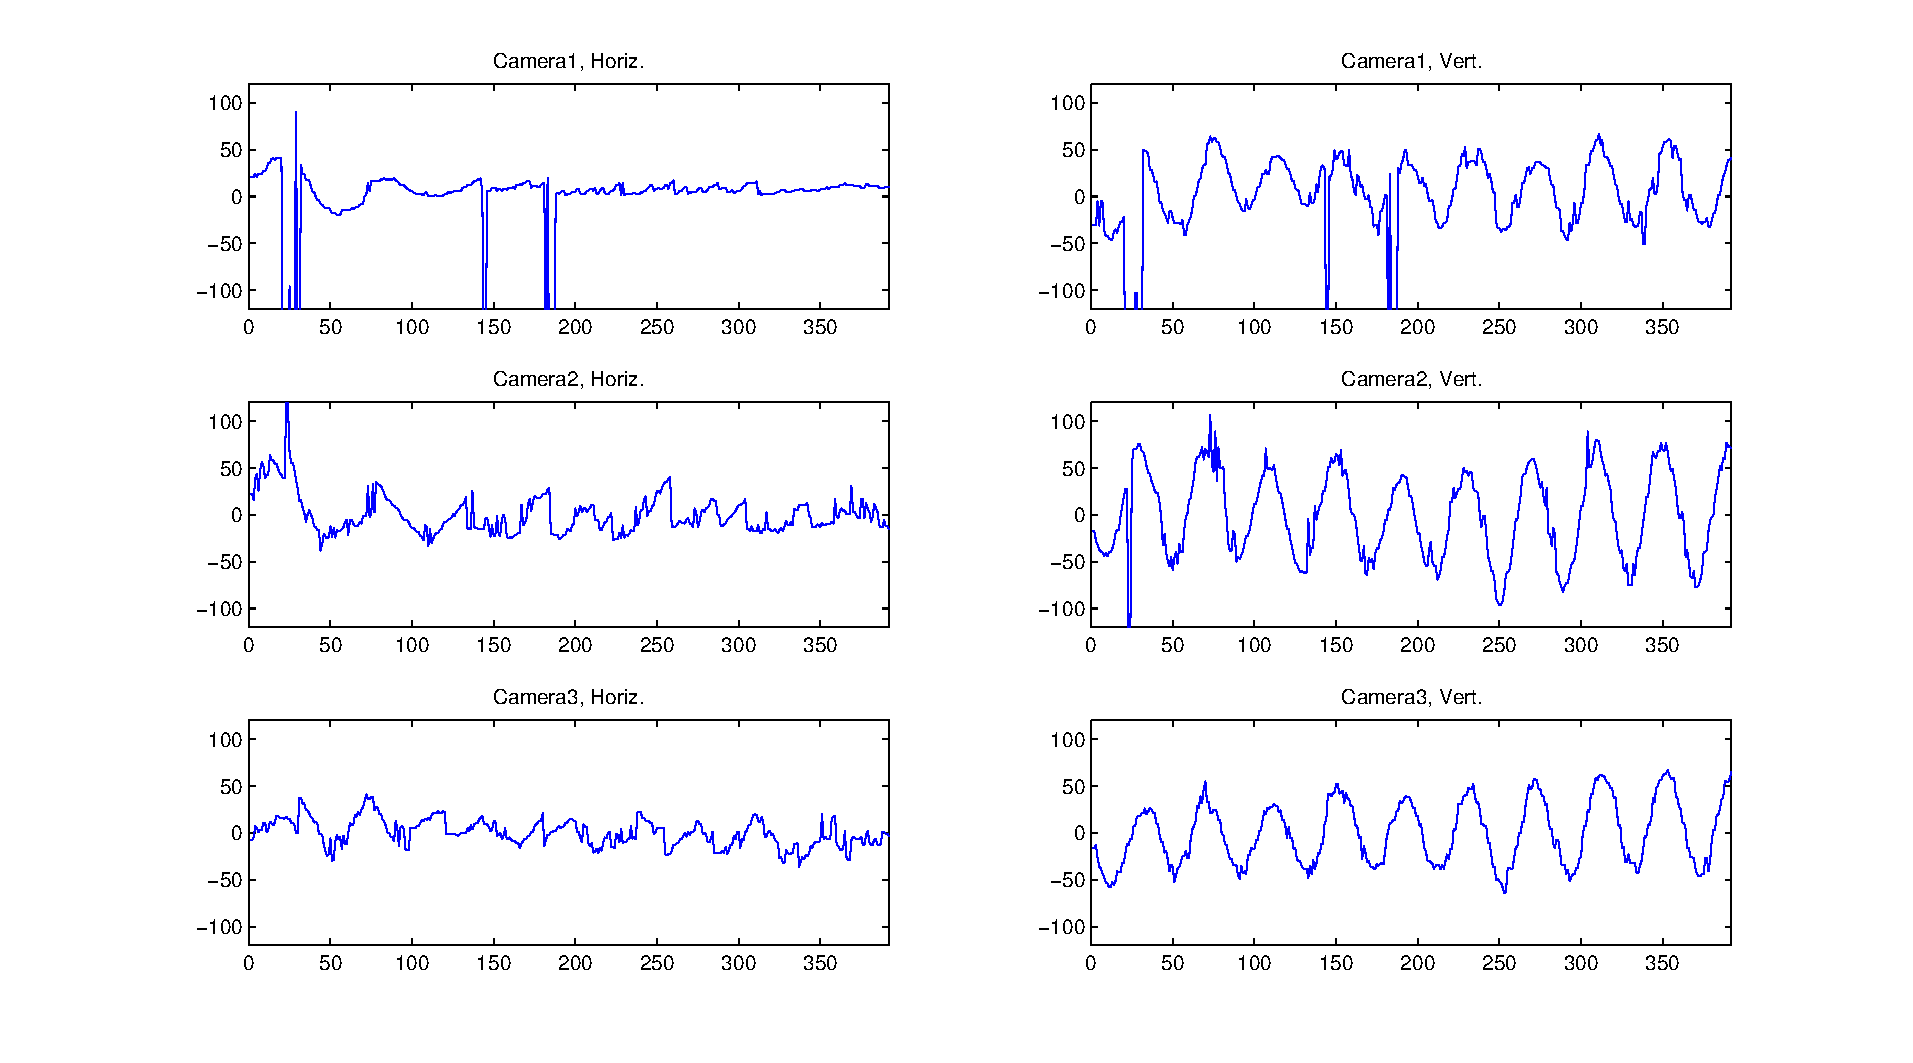
\includegraphics[width=1\columnwidth]{plots/test4_tracking}\textbf{}\\
\textbf{}%
\begin{minipage}[t]{0.75\columnwidth}%
\textbf{Figure 15.} For Test 4, the raw location tracking data shows
clear oscillation in the vertical (right) direction and erratic oscillation
in the horizontal (left) for all three cameras.%
\end{minipage}
\par\end{center}

\noindent \begin{center}
\pagebreak{}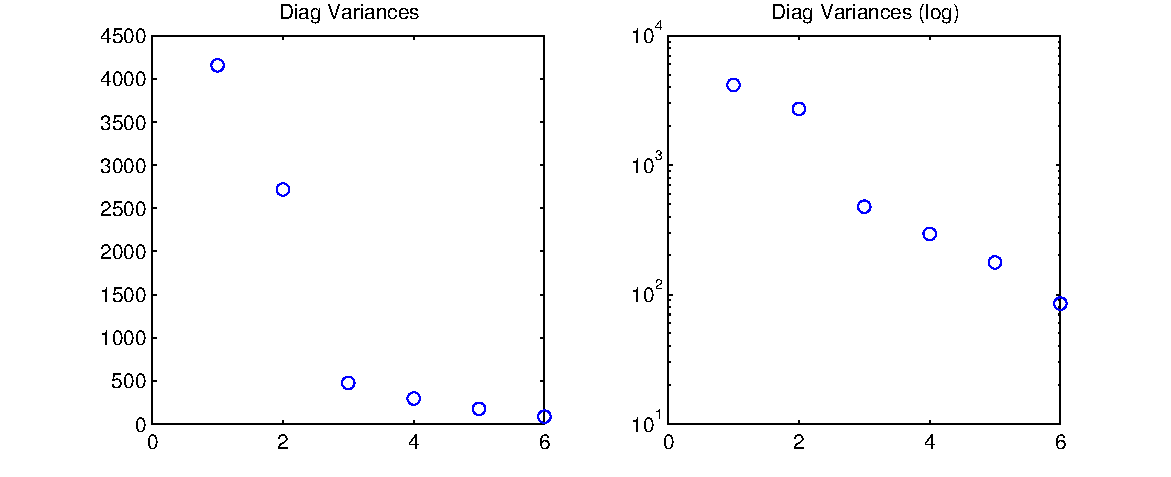
\includegraphics[width=0.95\columnwidth]{plots/test4_variance}\textbf{}\\
\textbf{}%
\begin{minipage}[t]{0.75\columnwidth}%
\textbf{Figure 16.} For Test 4, the diagonal variances $\left(\sigma_{i}^{2}=\lambda_{i}\right)$
show that the variance in the first two components are dominant but
that the trend is approximately linear for the six modes. %
\end{minipage}\vspace{0.03\paperheight}
\par\end{center}

\noindent \begin{center}
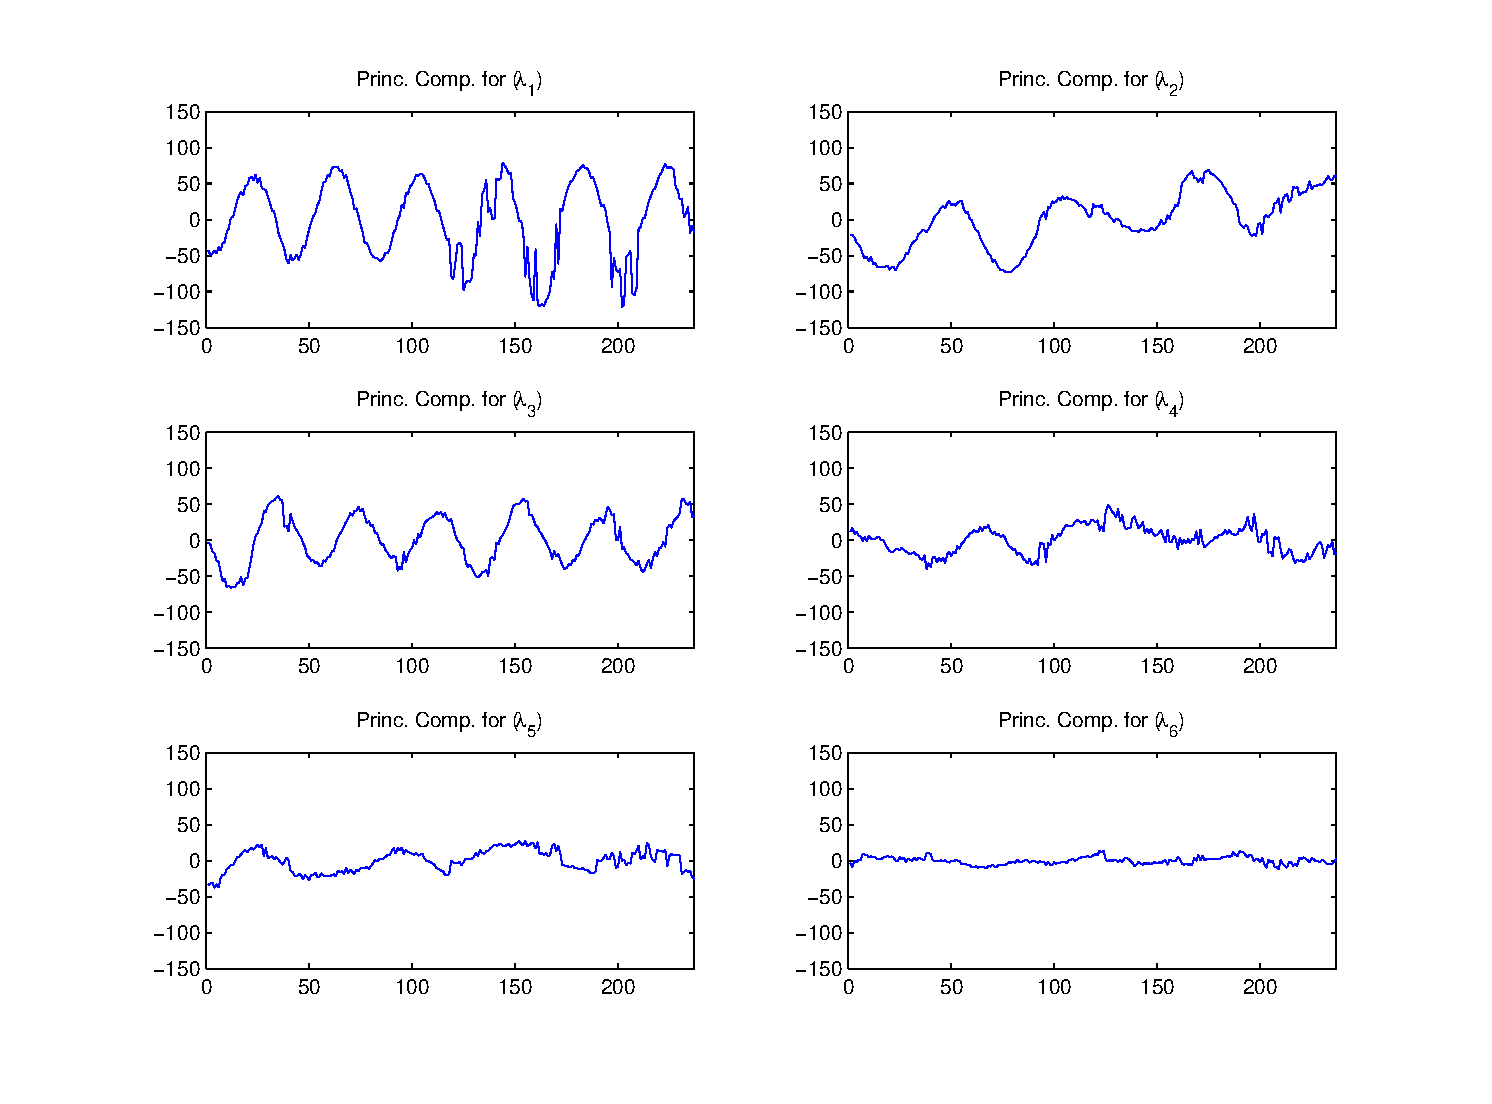
\includegraphics[width=0.95\columnwidth]{plots/test3_princComp}\textbf{}\\
\textbf{}%
\begin{minipage}[t]{0.75\columnwidth}%
\textbf{Figure 17.} For Test 4, the principal component projections
$\left(Y\right)$ shows that the first four or five components contain
oscillatory behavior.%
\end{minipage}
\par\end{center}

\noindent \begin{center}
\pagebreak{}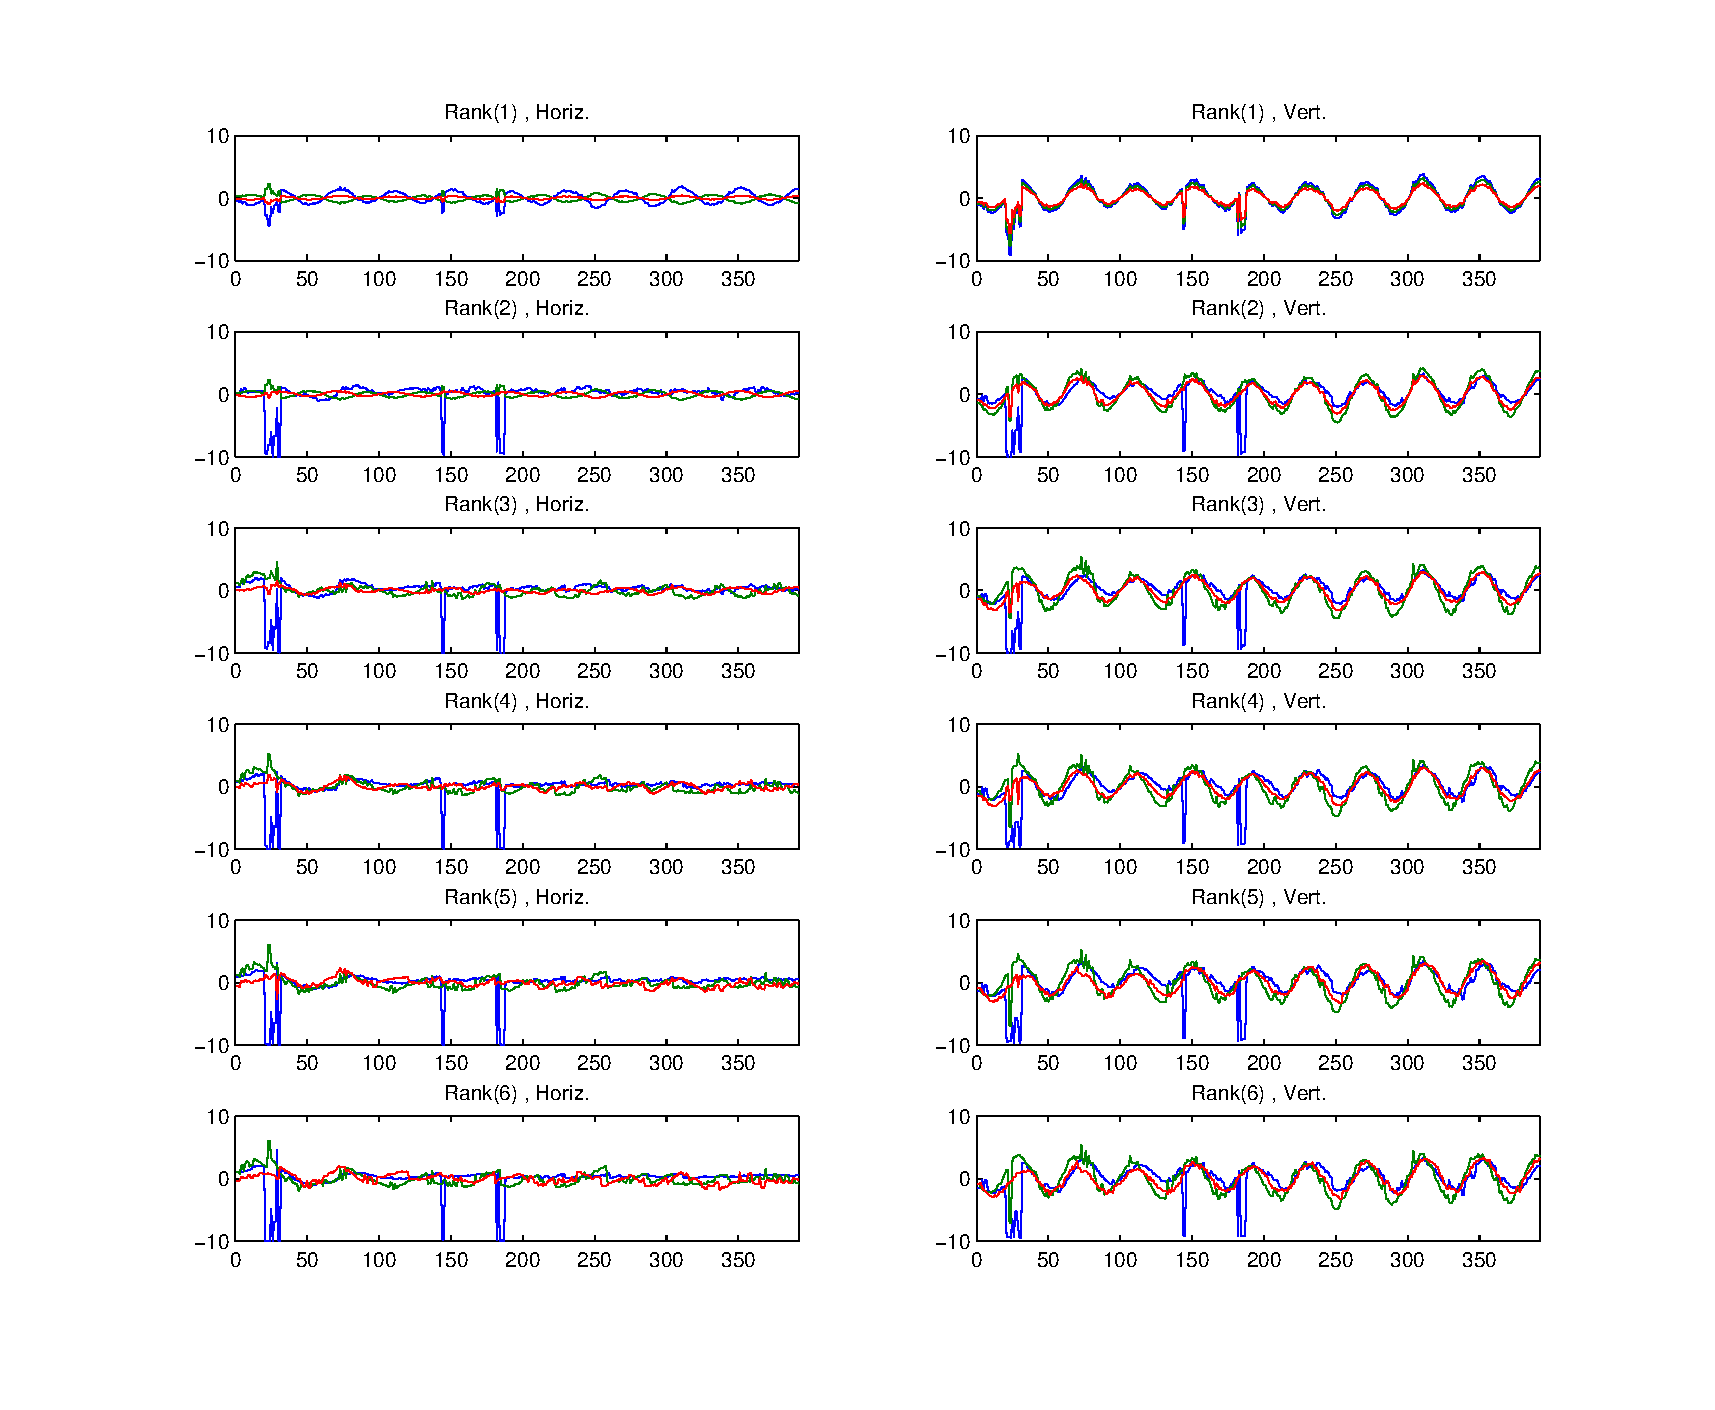
\includegraphics[width=0.85\columnwidth]{plots/test4_modes}\\
\textbf{}%
\begin{minipage}[t]{0.75\columnwidth}%
\textbf{Figure 18.} For Test 4, the proper orthogonal modes show that
a rank two approximation (second from top) captures the vertical and
horizontal oscillation and is a decent match to the full rank (bottom
row) data.%
\end{minipage}
\par\end{center}

\noindent \begin{center}
\vspace{0.05\paperheight}
\par\end{center}

\section{Summary and Conclusions}

Ultimately, this project shows that principal component analysis (PCA)
can be used to reduce redundancy and find directions of maximal variance
in complex data. This allows low rank approximations of multidimensional
dynamical behavior. One of the primary obstacles encountered was the
measurement of the paint can location in the video frames. This algorithm
adopts a suggestion from a classmate to track the yellow color on
the paint can. As with any experiment, experimental precision is critical
to minimizing error attributable to the procedure. I suspect some
of the erratic behavior, especially in Test 4 with the rotation, may
be the result of errors with the location tracking algorithms. However,
the paint can apparatus and the videography were not necessarily set
up for precision measurement and all of the observed results match
expected behavior with reasonable accuracy indicating the tracking
algorithm used was sufficient for the purposes of this project.

\noindent \begin{center}
\pagebreak{}
\par\end{center}

\section*{Appendix A}
\begin{description}
\item [{diag}] Used to extract the diagonals from a matrix.
\item [{double}] Used to convert 8-bit integer image data to double precision
format.
\item [{frame2im}] Used to covert a movie frame to an image.
\item [{imshow}] Used to plot image data.
\item [{load}] Loads data from an external file.
\item [{ind2sub}] Used to convert a linear index (in this case the minimum
value in the difference image) into corresponding 2D subscripts.
\item [{linspace}] Used to build a linear vector with $n+1$ points for
the spatial domain. The vector is then trimmed to $n$ points due
to the periodic boundaries.
\item [{mean}] Used to calculate the mean for each row of the location
coordinate data. 
\item [{min}] Used to find the minimum value in a given array.
\item [{num2str}] Used to convert a number to a string.
\item [{plot}] Used to plot the various parameters agains time or frequency.
\item [{repmat}] Used to replicate and tile an array for the means.
\item [{reshape}] Reshapes vector or matrix for given dimensions.
\item [{semilogy}] Used to make a plot with the $y$-axis on a logarithmic
scale.
\item [{size}] Used to get the number of rows and columns for a given matrix.
\item [{strcat}] Used to concatenate a string.
\item [{subplot}] Used to produce plot arrays.
\item [{sum}] Used to calculate sums.
\item [{switch}] Conditional structure used to vary code execution based
on a specified tag.
\item [{tic/toc}] Used to time the operations.
\item [{uint8}] Used to convert data to 8-bit integer format.
\item [{zeros}] Used to build vectors and matrices filled with ``0''.
\end{description}
\noindent \begin{center}
\pagebreak{}
\par\end{center}

\section*{Appendix B}

See project root for files (MATLAB) .
\begin{itemize}
\item Main script for this project = $\mathtt{main.m}$
\item $\mathtt{loadMovie.m}$
\item $\mathtt{playMovie.m}$
\item $\mathtt{plotProjections.m}$
\item $\mathtt{plotShifted.m}$
\item $\mathtt{plotTracking.m}$
\item $\mathtt{targetColor.m}$
\end{itemize}
\noindent 

\noindent \begin{center}
\vspace{0.01\paperheight}
\par\end{center}

\section*{Appendix C}

\subsubsection*{Diagonalization of the Covariance Matrix:}

The SVD for the matrix of the paint can locations is defined,
\[
X=U\Sigma V^{*}
\]
with the transformation variable defined,
\[
Y=U^{*}X\,.
\]
The covariance matrix of $Y$ is defined,
\[
C_{Y}=\frac{1}{n-1}YY^{T}=\frac{1}{n-1}\left(U^{*}X\right)\left(U^{*}X\right)^{T}=\frac{1}{n-1}U^{*}XX^{T}U
\]
and solving the eigenvalue problem,
\[
XX^{T}U=U\Sigma^{2}
\]
gives,
\[
C_{Y}=\frac{1}{n-1}U^{*}U\Sigma^{2}=\frac{1}{n-1}\Sigma^{2}\,.
\]

\end{document}
